\documentclass{article}

\usepackage{palatino}
\usepackage{graphicx}
\title{CS287: Natural Language Processing}
\pagenumbering{gobble}
\date{}
\begin{document}


\begin{figure}[c!]
  \centering
  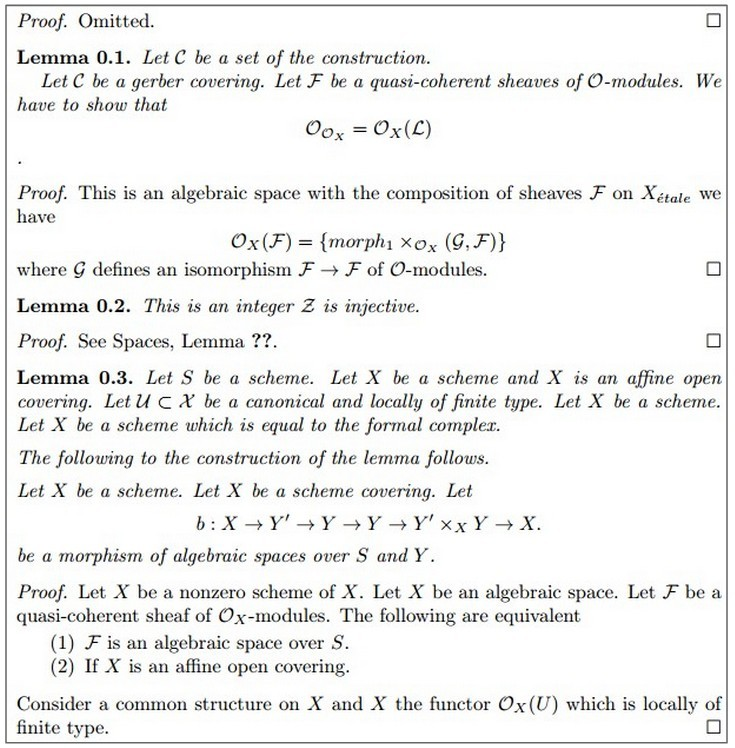
\includegraphics[width=1\linewidth]{latex3}

\vspace{1cm}
\begin{center}
\begin{center}
  {\huge Learn Algebraic Geometry$^*$}
\end{center}
\vspace{1cm}

 {\LARGE CS287: Natural Language Processing}
 \vspace{0.25cm}

 {\LARGE Tues/Thurs 2:30-4}
 \vspace{0.25cm}

 {\LARGE cs287.fas.harvard.edu}

\vspace{3cm}
{\footnotesize $^*$Hallucinated latex generated by an LSTM language model trained on the Stacks project. From \textit{The Unreasonable Effectiveness of Recurrent Neural Networks}  (http://karpathy.github.io/2015/05/21/rnn-effectiveness/)}

\end{center}

\end{figure}


\end{document}


